\documentclass[aspectratio=169,11pt]{beamer}

\usetheme{default}
\usecolortheme{dove}
\setbeamertemplate{navigation symbols}{}
\setbeamertemplate{footline}[frame number]
\setbeamercolor{frametitle}{fg=black}
\setbeamercolor{title}{fg=black}
\setbeamercolor{block title}{bg=blue!15,fg=black}
\setbeamercolor{block body}{bg=blue!5}
\setbeamercolor{block title example}{bg=green!15,fg=black}
\setbeamercolor{block body example}{bg=green!5}

\usepackage{tikz}
\usetikzlibrary{
  arrows.meta,
  positioning,
  shapes.geometric,
  fit,
  backgrounds,
  calc,
  decorations.pathmorphing
}
\usepackage{booktabs}
\usepackage{array}
\usepackage{adjustbox}

\title{Bayesian Approaches to Intuitive Physics}
\subtitle{Tenenbaum's Intuitive Physics Engine vs.\ pprim-probprog}
\author{}
\date{}

\begin{document}

% ──────────────────────────────────────────────
% TITLE
% ──────────────────────────────────────────────
\begin{frame}
\titlepage
\end{frame}

% ──────────────────────────────────────────────
% SLIDE 1 — Tenenbaum IPE
% ──────────────────────────────────────────────
\begin{frame}{Tenenbaum et al.\ --- Intuitive Physics Engine (IPE)}
\vspace{-2mm}
\begin{center}
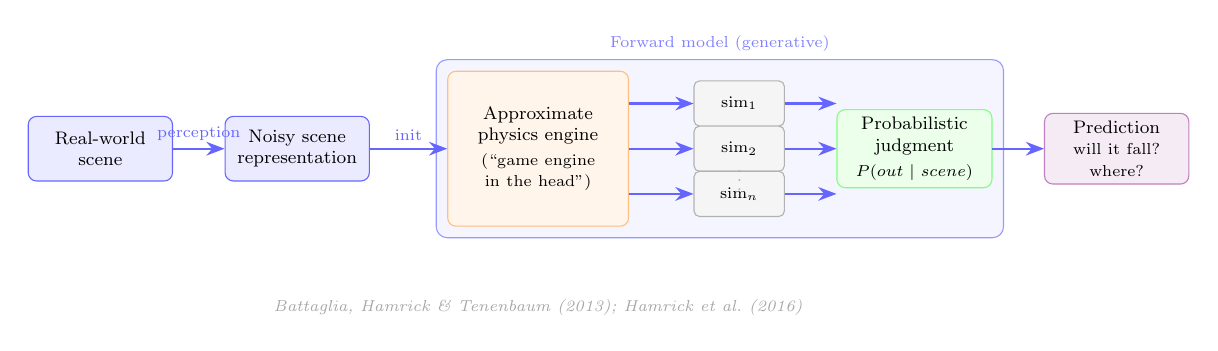
\begin{tikzpicture}[
    scale=0.82, every node/.style={transform shape},
    >=Stealth,
    node distance=6mm and 8mm,
    box/.style={
      rectangle, rounded corners=3pt, draw=blue!60, fill=blue!8,
      minimum height=10mm, minimum width=22mm,
      font=\footnotesize, align=center, text width=20mm
    },
    smallbox/.style={
      rectangle, rounded corners=2pt, draw=gray!60, fill=gray!8,
      minimum height=7mm, minimum width=14mm,
      font=\scriptsize, align=center
    },
    bigbox/.style={
      rectangle, rounded corners=4pt, draw=blue!40, fill=blue!4,
      inner sep=4pt
    },
    arr/.style={->, thick, blue!60},
    note/.style={font=\scriptsize\itshape, text=gray!70, align=center},
  ]

  % ── Perception ──
  \node[box] (scene) {Real-world\\scene};
  \node[box, right=8mm of scene] (percept) {Noisy scene\\representation};
  \draw[arr] (scene) -- node[above, font=\scriptsize] {perception} (percept);

  % ── Physics Engine ──
  \node[box, right=12mm of percept, minimum height=24mm, minimum width=28mm,
        fill=orange!8, draw=orange!50] (ipe)
    {Approximate\\physics engine\\[1mm]{\scriptsize(``game engine\\in the head'')}};
  \draw[arr] (percept) -- node[above, font=\scriptsize] {init} (ipe);

  % ── Monte Carlo sims ──
  \node[smallbox, right=10mm of ipe, yshift=7mm]  (sim1) {sim$_1$};
  \node[smallbox, right=10mm of ipe, yshift=0mm]  (sim2) {sim$_2$};
  \node[smallbox, right=10mm of ipe, yshift=-7mm] (simn) {sim$_n$};
  \node[note] at ($(sim2)!0.55!(simn)$) {$\vdots$};

  \draw[arr] (ipe.east |- sim1) -- (sim1);
  \draw[arr] (ipe.east |- sim2) -- (sim2);
  \draw[arr] (ipe.east |- simn) -- (simn);

  % ── Aggregation ──
  \node[box, right=8mm of sim2, fill=green!8, draw=green!50,
        minimum width=24mm] (judge)
    {Probabilistic\\judgment\\[0.5mm]{\scriptsize$P(\text{out} \mid \text{scene})$}};

  \draw[arr] (sim1.east) -- (judge.west |- sim1);
  \draw[arr] (sim2.east) -- (judge.west);
  \draw[arr] (simn.east) -- (judge.west |- simn);

  % ── Output ──
  \node[box, right=8mm of judge, fill=violet!8, draw=violet!50] (out)
    {Prediction\\[0.5mm]{\scriptsize will it fall?\\where?}};
  \draw[arr] (judge) -- (out);

  % ── Annotation ──
  \node[note, below=10mm of ipe]
    {Battaglia, Hamrick \& Tenenbaum (2013); Hamrick et al.\ (2016)};

  % ── Background box ──
  \begin{scope}[on background layer]
    \node[bigbox, fit=(ipe)(sim1)(simn)(judge),
          label={[font=\scriptsize, text=blue!50]above:Forward model (generative)}] {};
  \end{scope}

\end{tikzpicture}
\end{center}

\begin{block}{Key idea}
Humans predict physics by running noisy, approximate \textbf{forward simulations}
and aggregating outcomes --- ``analysis by synthesis'' at the \emph{prediction} level.
\end{block}
\end{frame}

% ──────────────────────────────────────────────
% SLIDE 2 — pprim-probprog
% ──────────────────────────────────────────────
\begin{frame}{pprim-probprog --- Bayesian P-Prim Inference}
\vspace{-2mm}
\begin{center}
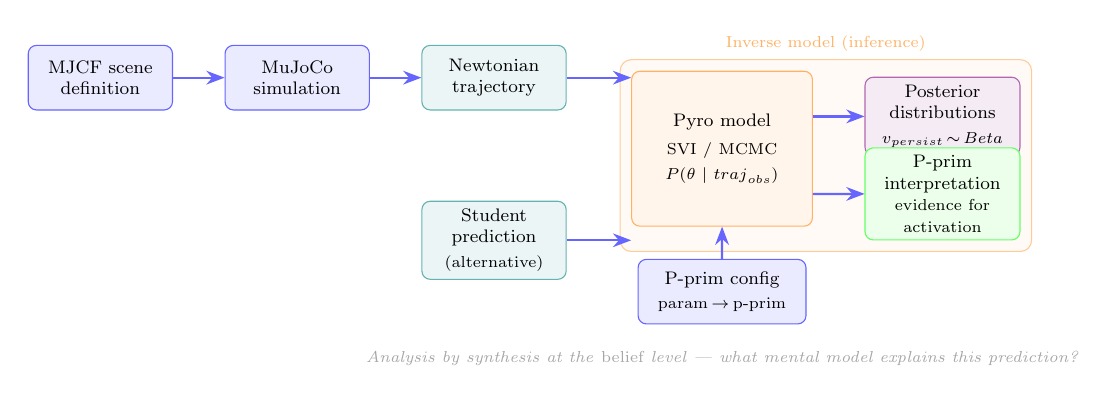
\begin{tikzpicture}[
    scale=0.82, every node/.style={transform shape},
    >=Stealth,
    node distance=6mm and 8mm,
    box/.style={
      rectangle, rounded corners=3pt, draw=blue!60, fill=blue!8,
      minimum height=10mm, minimum width=22mm,
      font=\footnotesize, align=center, text width=20mm
    },
    databox/.style={
      rectangle, rounded corners=3pt, draw=teal!60, fill=teal!8,
      minimum height=10mm, minimum width=22mm,
      font=\footnotesize, align=center, text width=20mm
    },
    inferbox/.style={
      rectangle, rounded corners=3pt, draw=orange!60, fill=orange!8,
      minimum height=10mm, minimum width=22mm,
      font=\footnotesize, align=center, text width=20mm
    },
    resultbox/.style={
      rectangle, rounded corners=3pt, draw=violet!60, fill=violet!8,
      minimum height=10mm, minimum width=22mm,
      font=\footnotesize, align=center, text width=20mm
    },
    bigbox/.style={
      rectangle, rounded corners=4pt, draw=orange!40, fill=orange!4,
      inner sep=4pt
    },
    arr/.style={->, thick, blue!60},
    note/.style={font=\scriptsize\itshape, text=gray!70, align=center},
  ]

  % ── Top row: simulation ──
  \node[box] (mjcf) {MJCF scene\\definition};
  \node[box, right=8mm of mjcf] (mujoco) {MuJoCo\\simulation};
  \draw[arr] (mjcf) -- (mujoco);

  \node[databox, right=8mm of mujoco] (newton) {Newtonian\\trajectory};
  \draw[arr] (mujoco) -- (newton);

  % ── Bottom row: student prediction ──
  \node[databox, below=14mm of newton] (student)
    {Student\\prediction\\[0.5mm]{\scriptsize(alternative)}};

  % ── Inference engine ──
  \node[inferbox, right=10mm of newton, yshift=-11mm,
        minimum height=24mm, minimum width=28mm] (pyro)
    {Pyro model\\[1mm]{\scriptsize SVI / MCMC}\\[0.5mm]{\scriptsize$P(\theta \mid \text{traj}_\text{obs})$}};

  \draw[arr] (newton.east) -- (pyro.west |- newton);
  \draw[arr] (student.east) -- (pyro.west |- student);

  % ── Posterior ──
  \node[resultbox, right=8mm of pyro, yshift=5mm,
        minimum width=24mm] (posterior)
    {Posterior\\distributions\\[0.5mm]{\scriptsize$v_\text{persist} \!\sim\! \text{Beta}$}};
  \draw[arr] (pyro.east |- posterior) -- (posterior);

  % ── Interpretation ──
  \node[resultbox, right=8mm of pyro, yshift=-7mm,
        minimum width=24mm, draw=green!60, fill=green!8] (interp)
    {P-prim\\interpretation\\[0.5mm]{\scriptsize evidence for\\activation}};
  \draw[arr] (pyro.east |- interp) -- (interp);

  % ── Config ──
  \node[box, below=5mm of pyro, minimum width=26mm] (config)
    {P-prim config\\[0.5mm]{\scriptsize param $\!\to\!$ p-prim}};
  \draw[arr] (config) -- (pyro);

  % ── Background ──
  \begin{scope}[on background layer]
    \node[bigbox, fit=(pyro)(posterior)(interp),
          label={[font=\scriptsize, text=orange!60]above:Inverse model (inference)}] {};
  \end{scope}

  % ── Annotation ──
  \node[note, below=3mm of config]
    {Analysis by synthesis at the \emph{belief} level --- what mental model explains this prediction?};

\end{tikzpicture}
\end{center}

\begin{block}{Key idea}
Given an observed prediction, \textbf{infer the belief parameters} (e.g.\ velocity persistence)
that would generate it --- ``analysis by synthesis'' at the \emph{cognitive model} level.
\end{block}
\end{frame}

% ──────────────────────────────────────────────
% SLIDE 3 — Comparison table (part 1)
% ──────────────────────────────────────────────
\begin{frame}{Comparison}
\begin{center}
\renewcommand{\arraystretch}{1.12}
\scriptsize
\begin{tabular}{>{\raggedright\arraybackslash}p{2.2cm}
                >{\raggedright\arraybackslash}p{5.0cm}
                >{\raggedright\arraybackslash}p{5.0cm}}
\toprule
\textbf{Dimension}
  & \textbf{Tenenbaum IPE}
  & \textbf{pprim-probprog} \\
\midrule
\textbf{Central question}
  & How do people \emph{predict} physical outcomes?
  & What \emph{beliefs} best explain a given prediction? \\
\textbf{Direction}
  & Forward: scene $\to$ predicted outcome
  & Inverse: observed prediction $\to$ belief parameters \\
\textbf{Generative model}
  & Approximate Newtonian engine (``game engine in the head'')
  & Parameterized physics model (velocity persistence, force scaling, \ldots) \\
\textbf{Inference}
  & Monte Carlo forward simulation; aggregate samples
  & Pyro SVI (variational) or MCMC/NUTS over posterior \\
\textbf{Simulator}
  & Abstract / hypothesized mental engine
  & MuJoCo (ground-truth Newtonian reference) \\
\textbf{What varies}
  & Perceptual noise, simulation stochasticity
  & Belief parameters ($v_{\text{persist}}$, force scaling, \ldots) \\
\textbf{Output}
  & Probability of physical outcomes
  & Posterior over cognitive params + p-prim interpretation \\
\textbf{Theory}
  & Rational analysis / Bayesian cognitive science
  & P-prims (diSessa, 1993); knowledge-in-pieces \\
\textbf{Unit of analysis}
  & The prediction itself
  & The \emph{generating belief} behind the prediction \\
\textbf{View of errors}
  & Noise + approximate simulation
  & Alternative predictions reflect \emph{productive} intuitive knowledge \\
\midrule
\textbf{Shared basis}
  & \multicolumn{2}{>{\raggedright\arraybackslash}p{10.2cm}}{Both use \textbf{Bayesian analysis-by-synthesis}: posit a generative process, use probabilistic inference to connect observations to latent variables. They differ in \emph{what} is latent --- physical outcomes (IPE) vs.\ cognitive parameters (pprim-probprog).} \\
\bottomrule
\end{tabular}
\end{center}
\end{frame}

\end{document}
